\documentclass[article,oneside]{memoir}

\usepackage{amsmath}
\usepackage{amssymb}
\usepackage{cclicenses}
\usepackage{color}
\usepackage{euler}
\usepackage[colorlinks=true,linkcolor=blue,citecolor=red]{hyperref}
\usepackage{float}
\usepackage{framed}
\usepackage[letterpaper,margin=2.5cm]{geometry}
\usepackage{graphicx}
\usepackage{indentfirst}
\usepackage{lipsum}
\usepackage{longtable}
\usepackage[final]{microtype}
\usepackage{multicol}
\usepackage{nameref}
\usepackage{pdflscape}
\usepackage{pdfpages}
\usepackage{tabularx}
\usepackage{textcomp}
\usepackage{todonotes}
\usepackage{libertine}
\usepackage{inconsolata}
\usepackage{upgreek}
%\usepackage{mathptmx} % <-- Times font


% PAGE SETUP
\setlength{\parindent}{5mm}
\nonzeroparskip
\raggedbottom
\raggedcolumns

% CONFIG FOR TOC, BIBLIO, ETC
\setcounter{secnumdepth}{5}
\setcounter{tocdepth}{2}
\renewcommand{\bibname}{References}
\renewcommand{\abstractname}{Executive Summary}
\renewcommand{\contentsname}{Table of Contents}

% HANDY DEFINITIONS
\newcommand{\note}[1]{ \begin{framed} #1 \end{framed} }
\newcommand{\refdes}[1]{\texttt{#1}}
\newcommand{\mr}[1]{\ensuremath{\mathrm{#1}}}
\newcommand{\dg}{\ensuremath{{}^\circ}}
\newcommand{\schematicpage}[2]{ \begin{framed} Relevant schematic page: \hyperlink{schematic.pdf.#1}{\texttt{#2/#1}} \end{framed} }
\newcommand{\greylipsum}[1]{{\color{gray} \lipsum[#1]}}
\newcommand{\kOhm}{\ensuremath{\mathrm{k}\Omega}}
\newcommand{\Ohm}{\ensuremath{\Omega}}
\newcommand{\Pos}[1]{{\ensuremath{+}#1}}
\newcommand{\Neg}[1]{{\ensuremath{-}#1}}
\newcommand{\uA}{\ensuremath{\upmu\mathrm{A}}}
\newcommand{\uF}{\ensuremath{\upmu\mathrm{F}}}
\newcommand{\uV}{\ensuremath{\upmu\mathrm{V}}}

\title{Design Report}
\author{WCP52}

\begin{document}

\pagestyle{headings}
\begin{titlingpage}
%\setlength\extrarowheight{10mm}
\begin{tabularx}{\textwidth}{Xr}
\hline
\\
{\LARGE OWNER'S AND SERVICE MANUAL} &
Gain/Phase Analyzer \\
\\
\hline
\end{tabularx}
\vfill
\begin{center}
\missingfigure[figwidth=4in]{Photo}
\end{center}
\vfill
\begin{center}
\textcopyright 2015, WCP52. Licensed under a Creative Commons Attribution 4.0 International License.
\end{center}
\end{titlingpage}

%\begin{multicols}{2}

\begin{abstract}
In the current market, electronics lab equipment that can analyze a frequency
response by gain and phase (a vector analyzer) is very expensive, often
reaching into the tens of thousands of dollars.  They are large, heavy
instruments, and are not portable between home, class and a lab. A direct
result of this high cost is that they are generally unobtainable for teachers
to use in classrooms and labs to enhance their education techniques and for
students to use as a hands-on tool for circuit analysis projects.  Due to their
lack of portability, those teachers who do have access to a vector analyzer can
not use its vast functionality for demonstrations of a circuit's behavior in
front of a classroom or in a lab with many students.

It is our goal to remedy this situation by creating a low cost, portable device
that can provide an analysis of gain and phase in a graph.  

This gain/phase analyzer can be produced and sold for approximately \$100. The
device is portable and can be carried between home, work, labs, classrooms, etc
and is very easy to set up with a USB connection to a computer and a power
outlet.  

Additionally, our device is an open source project, with all hardware and
software source available online.  Thus, any capable students or engineers will
have ability to learn how it works and modify the design any way they choose.
This can be a great way for students to gain some hands-on experience in
learning some advanced circuit design techniques and microcontroller
programming.  Additionally, one can apply one’s own creativity and ingenuity to
improve the design of this project; making a better device for future teachers
and students. 
\end{abstract}


\newpage
\tableofcontents*
%\listoffigures

\newpage
\chapter{Problem Definition}

Tools such as vector analyzers are heavy and expensive, costing tens of
thousands of dollars.  There is need of a tool for students and teachers to
help teach electronics and similar courses.  Currently, there are no feasibly
affordable tools to show the frequency response and phase of a circuit,
amplifier, or control loop, and the learning experience is hindered by this
gap.

\section{Problem Scope}

This project will produce a portable frequency response analyzer.  It will
communicate data with a computer through USB in order to form a Bode plot of
the frequency and phase response of the circuit.

\section{Technical Review}

Proper circuit analysis is a fundamental practice in the field of engineering,
since it is necessary for every electronic device on the market.  As a result,
it is the goal of every engineering institution to give students a strong basis
in circuit design and analysis.

Currently, this is done mainly through lecture and labs.  A professor stands in
front of a classroom and delivers a lecture based on PowerPoint slides that
they have created.  It is expected that, from this, students grasp the concepts
necessary to make them proficient in working with electronics.  Although this
may be a seemingly efficient way to broadcast the fundamentals to many people,
it must be augmented with practice.

Then, there is the lab section of the class.  Students are asked to put
together a circuit and then observe it using a measuring device. Unfortunately,
few such devices are available for frequency-domain work.

It is the goal of this project to help remedy this situation.  This USB
Gain/Phase Analyzer is a cheap, portable tool.  With this, a teacher would have
the ability to bring circuits to class and actually demonstrate fundamentals to
their students.  This would inevitably enhance the effectiveness of their
lectures because students would see how these circuits respond in application.
The aim, here, is to help a teacher captivate his/her students.

Additionally, the analyzer is a tool that students can afford.  In a lab, they
could now be asked to design something, increasing the creative thinking of the
prospective engineer.  With this tool, they can now do more meaningful analysis
and see their devices' behaviors on real world signals.  Also, the device is
portable enough that students could take it home and do lab work there, without
needing to spend thousands of dollars on lab equipment.

\section{Design Requirements}

\subsection{Context-Level Constraints}

This project is producing one gain/phase analyzer system. As shown in \autoref{fig:contextdiag},
 the device connects to a PC for user control and viewing of data. It has one
Drive output, with which it applies a stimulus to a Device Under Test (DUT),
and two Sense inputs, with which it detects the amplitude and phase of signals
before and after the DUT. The device will also have an Adapter port, with which
it can connect to external adapters for measuring various types of DUTs.  The
gain/phase analyzer system, in addition to the hardware, comprises PC Software
with which the end user may start analyses and view results.

\begin{figure}[H]
\centering
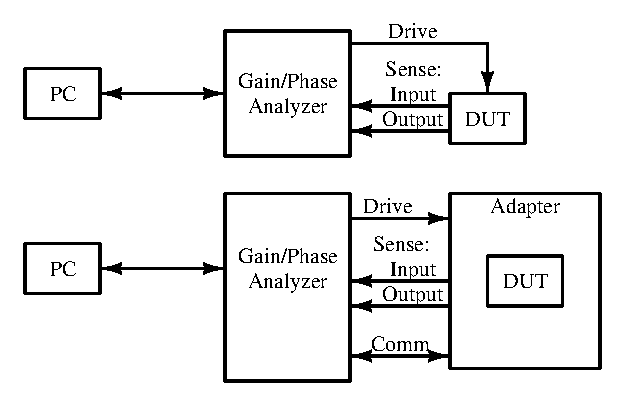
\includegraphics{contextdiagram}
\caption{Gain/Phase Analyzer Context Diagram}
\label{fig:contextdiag}
\end{figure}

\subsection{System-Level Constraints}

As shown in \autoref{fig:systemdiag}, the analyzer uses a \emph{Synthesizer} to
generate the stimulus signal, and an \emph{Output Amplifier} to provide the stimulus
signal to the DUT, at up to 1.25 V RMS and up to 150 MHz. \emph{Input Filters}, an
\emph{Input Switching Network} and the \emph{Input Detector} provide a signal corresponding
to the amplitude of the signals at the Sense ports. The Input Switching Network
can also select a \emph{Phase Reference} to be summed with the signals for phase
measurement. These are digitized by an \emph{Analog-Digital Converter} to be processed
by the \emph{Microprocessor}. The Microprocessor then interfaces with the \emph{Software} via
the \emph{PC Interface}.

\begin{figure}[H]
\centering
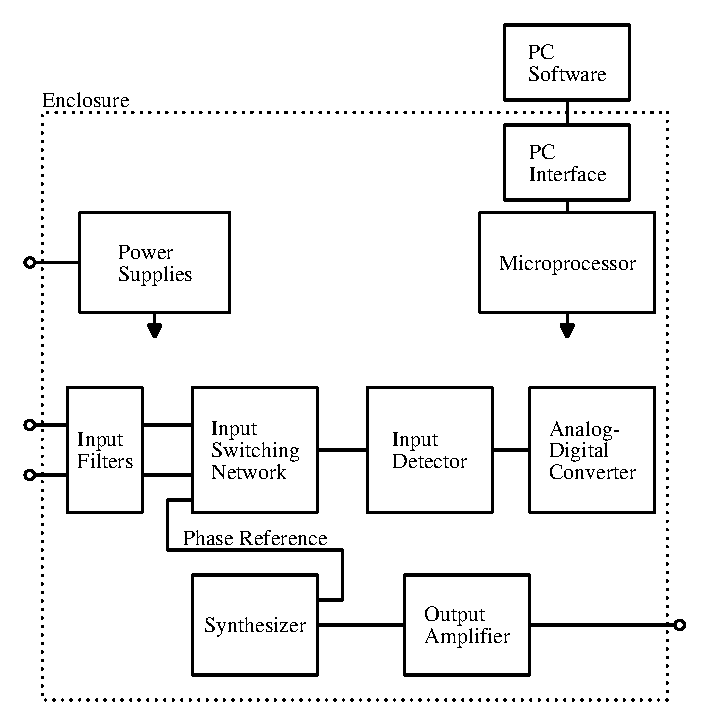
\includegraphics{systemdiagram}
\caption{Gain/Phase Analyzer System Diagram}
\label{fig:systemdiag}
\end{figure}

\chapter{Design Description}

\section{Overview}
A Gain/Phase Analyzer is an instrument used to plot the frequency response of a
network or amplifier. The project, sponsored by Professor Kyle Temkin,
specifies a small, computer controlled gain/phase analyzer for use by students
and individuals. It can stimulate and then measure filters, amplifiers and
control systems, allowing their behavior to be plotted and analyzed. The device
is to be developed as an open-source project, so that students may study its
inner workings.

\section{Detailed Description}
Our project lacks many various and viable implementation
possibilities. As such, many major decisions will involve study of other
instrumentation which performs similar tasks, including a few open-source
network analyzers. Trade study will be used as required for selecting high-cost
components or designs of subsystems, and this will be addressed as necessary
during the development cycle. Hardware is being designed and  implemented in
different stages in order to ease the process of design. Software will be
created with the purpose of interfacing with the microcontroller.

\subsection{Synthesizer}
The first subsystem that will be built is the frequency synthesizer. This needs
to generate a frequency up to $150\;\mr{MHz}$. For this design, the circuit uses
the AD9958 Direct Digital Synthesis (DDS) chip and a `video' op-amp to produce
the correct output.

\begin{figure}[H]
\centering
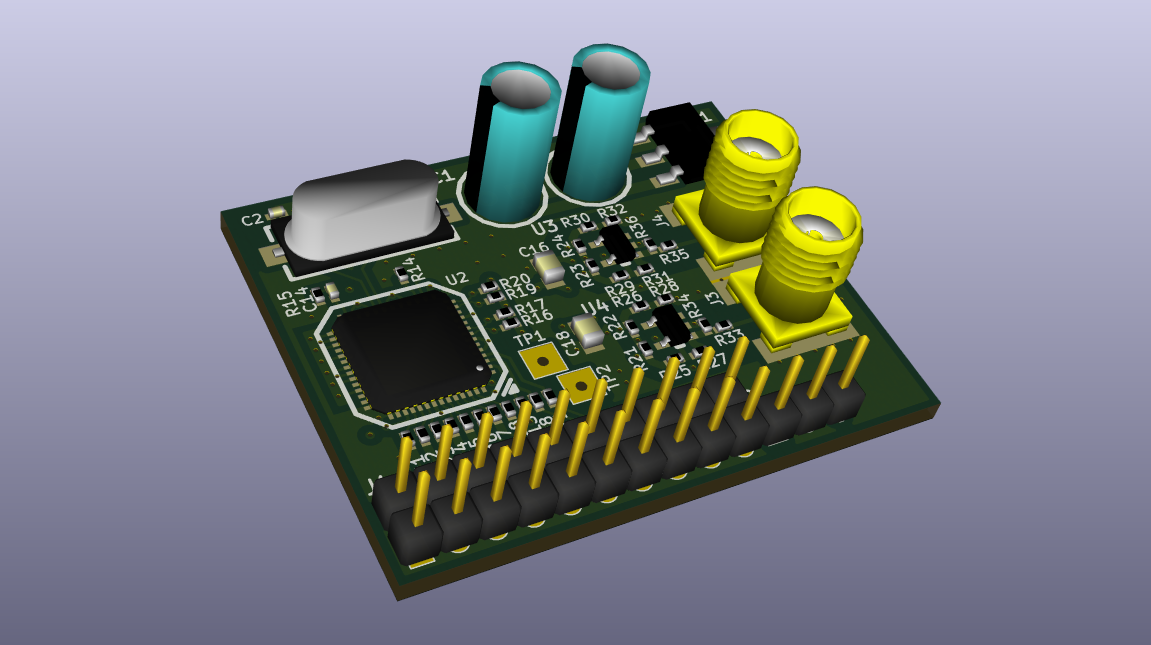
\includegraphics[width=4in]{synth3d.png}
\caption{Synthesizer PCB, 3D render}
\label{fig:synth3d}
\end{figure}

In the final product, we may integrate an optional CPLD or FPGA to allow the user
to drive the modulation feature of the DDS chip; for the purposes of testing we
have tied the modulation inputs straight to ground, as we do not require them.

\subsection{Input Front-end}
The next section of the design is the input front-end subsystem.

\begin{figure}[H]
\centering
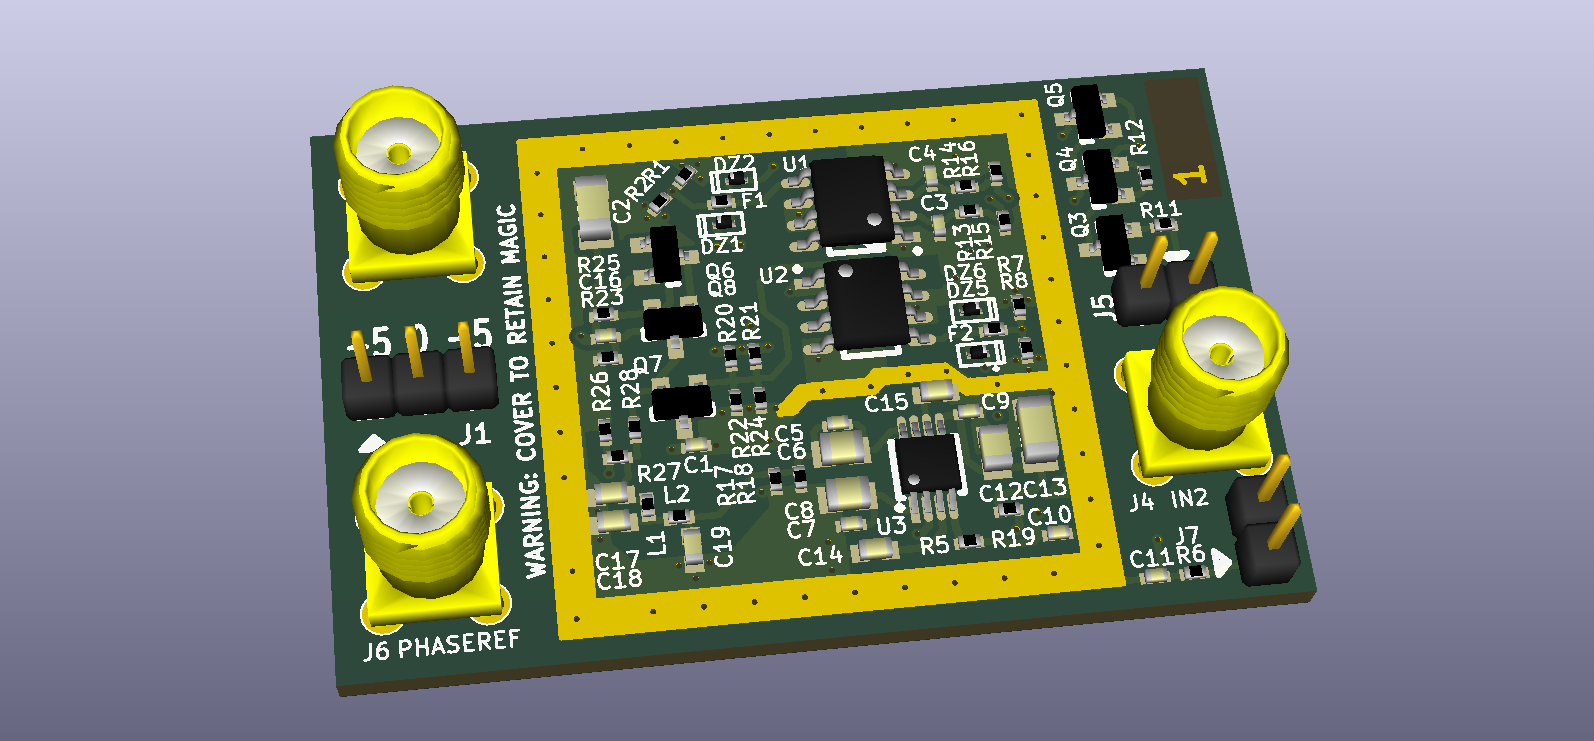
\includegraphics[width=4in]{frontend3d.png}
\caption{Input Front-end PCB, 3D render}
\label{fig:front3d}
\end{figure}

Our input front-end must take the signals from the front-panel input connectors
and present them in a form which can be directly sampled by the
microcontroller's analog-to-digital converter. The signals first pass through a
simple input protection circuit. This consists of a small-footprint SMD fuse in
series with the input and a clamping arrangement set around $3.3\;\mr{V}$
($23\;\mr{dBm}$ peak).  After the input protection, the two input signals enter
a switching circuit to select between them. This allows all of the following
circuitry to be shared between channels, minimizing cost and inter-channel
variation. This is followed by a buffer, which isolates the input signal from
the following power combiner and filter. After that, a power combiner adds in a
variable phase reference, which allows the system to measure the input signal's
phase, and a filter cuts the signal off at $300\;\mr{MHz}$. The filtered signal
then passes into a logarithmic detector with integrated low-pass filter, which
presents a voltage proportional to the logarithm of the input amplitude to the
microcontroller.

\subsection{Output Amplifier}
The next section of the design is the output amplifier subsystem.

\begin{figure}[H]
\centering
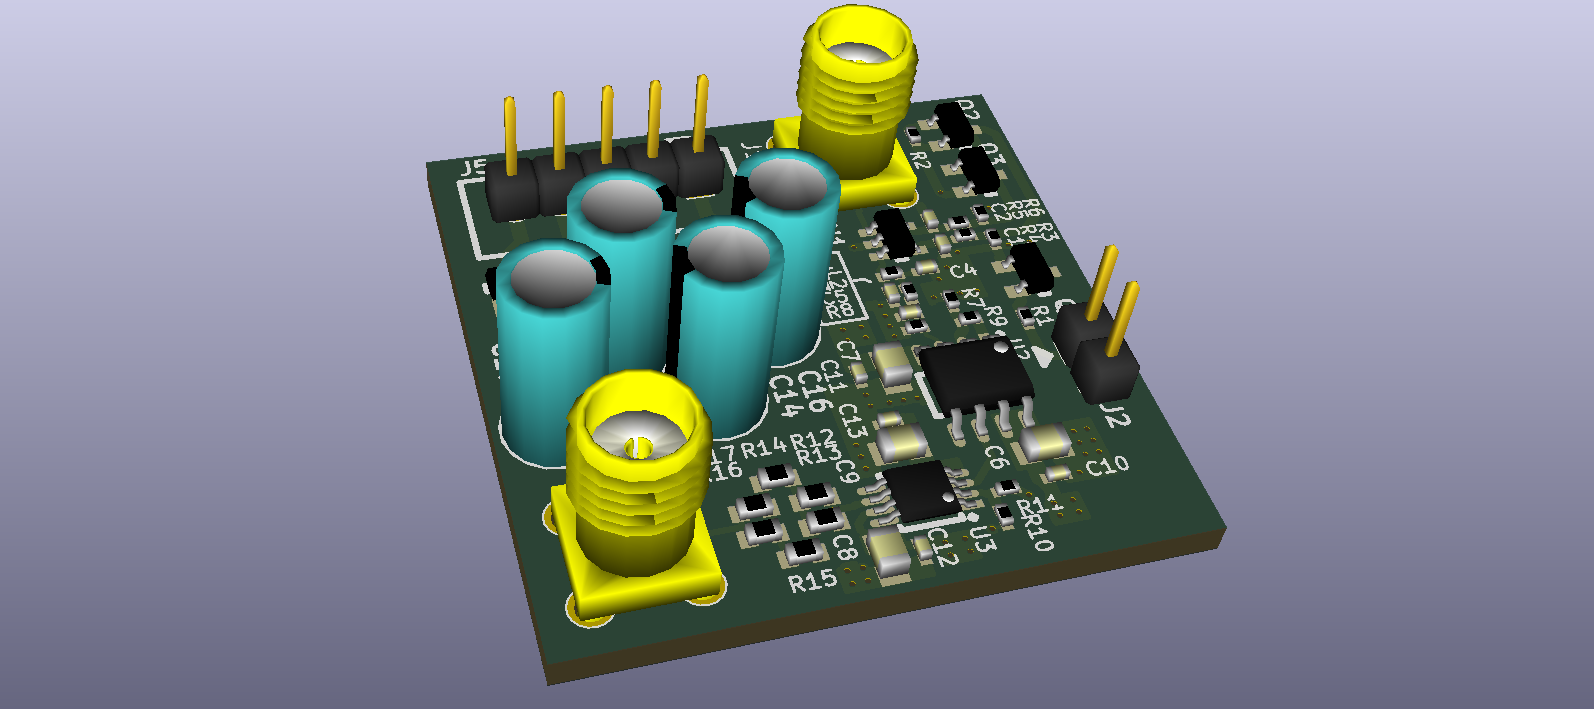
\includegraphics[width=4in]{outamp3d.png}
\caption{Output Amplifier PCB, 3D render}
\label{fig:outamp3d}
\end{figure}

The output amplifier must take small signals, at $–8.5\;\mr{dBm}$ as they arrive from
the synthesizer, and output the full $15\;\mr{dBm}$  signal. For design margin, a $16.5\;\mr dBm$
 output amplitude is assumed. This gives a required gain of $25\;\mr dB$. An
additional $6\;\mr dB$ gain is required to compensate for the insertion loss of the
termination, giving a total required gain of $31\;\mr dB$.  A gain of $31\;\mr dB$ from $1\;\mr kHz$
(practically DC) to $150\;\mr MHz$ is difficult to achieve, particularly with the very
large absolute amplitude of $21\;\mr dBm$ at the output. We chose to use two gain
stages of $15.5\;\mr dB$ each. The final stage is a THS3001 operational amplifier, as
it supports the high slew rate, high voltage and high output current required.
This is a very expensive amplifier, though, so we used the AD8000 (similar
specifications, but with a lower maximum supply voltage) for the first stage.
The synthesizer allows amplitude control, but this control is applied at the
digital stage, resulting in a loss of DAC resolution. To get more range at full
resolution, we included a MAADSS0008 switchable $15\;\mr dB$ attenuator in the output
amplifier's signal path.

\subsection{Microprocessor}
For our system's microprocessor, we used the Atmel SAM4S16C ARM Cortex-M4
microcontroller. In the final product, we will switch to a less expensive
microcontroller in the SAM4S line with a smaller amount of memory, after we
have determined the amount needed.

In the current prototype, we are using the Atmel SAM4S Xplained evaluation kit;
the final product will use the chip by itself.

\section{Use}
The purpose of this device is provide students with tangible data when analyzing
circuits. As shown in \autoref{fig:contextdiag}, the device is to be connected between
a PC and a device under test; the user can initiate an analysis using the supplied software.

\chapter{Evaluation}

\section{Overview}
Our system was designed through a combination of computer simulation, and
prototype testing. After carefully designing each subsystem,
per-subsystem PCBs were fabricated and interconnected to build a prototype, which was
thoroughly tested before the final PCB was designed and fabricated.

As our project is a piece of electrical test equipment, the majority of the
tests are electrical in nature. The tests for requirements \hyperref[prs:3.2.2]{3.2.2}
and \hyperref[prs:3.2.3]{3.2.3} (output signal characteristics) require
an oscilloscope with at least $300$~MHz bandwidth. The remaining electrical
tests require only a basic multimeter, and often use the instrument to
verify itself. For example, \hyperref[prs:3.2.4]{3.2.4} (sensitivity) is
verified by measuring the reported amplitude from the output amplifier, and
comparing that to the input noise floor. Requirement \hyperref[prs:3.2.6]{3.2.6}
(accuracy) is verified by examining the normalized sweep of a flat-response
attenuator. Some requirements, for example \hyperref[prs:3.2.1]{3.2.1} (type
of plot), \hyperref[prs:3.3.1]{3.3.1 -- 3.3.3} (interface design), and \hyperref[prs:3.6.4]{3.6.4}
(direct control) are verified simply by observing how the instrument responds to
PC control. Others, for example \hyperref[prs:3.3.4]{3.3.4} (panel connectors),
\hyperref[prs:3.6.1]{3.6.1} (Operator's Manual), \hyperref[prs:3.6.2]{3.6.2} (Protocol Guide),
and \hyperref[prs:3.6.3]{3.6.3} (surface-mount technology) are verified by observing the
instrument and accompanying materials themselves.

The full project requirements can be found in \hyperref[chap:prs]{Appendix~\ref{chap:prs}}, and the full
test procedures can be found in \hyperref[chap:test]{Appendix~\ref{chap:test}}.

\section{Testing and Results}

The full test procedures can be found in Appendix~\ref{chap:test}.

%\note{As the full tests have not been performed at the time of this draft,
%\emph{Italicized} text is used as a placeholder for missing results.}

\subsection*{Requirement WCP52.3.1.1 --- Required mode: Idle}
This requirement simply means that the device must have a mode in which it is
not performing analysis. We measured the output signal in this state, and
demonstrated that the ``sample'' annunciator was not lit.

\textbf{Maximum output amplitude in ``idle'':} 6.0~mV~p-p, 750~\uV~RMS (mostly amplifier noise)

\subsection*{Requirement WCP52.3.1.2 --- Required mode: Analysis}
This requirement means that the device must have a non-idle mode in which it is
performing its primary function. This does not require a separate demonstration;
the fact that it performs correctly in the demonstration for WCP52.3.2.6 shows
that it must be capable of performing analysis.

\subsection*{Requirement WCP52.3.2.1 --- Bode plot}
By providing sample data to the PC software and causing it to display a
plot, we demonstrated that the software is capable of displaying a Bode plot.

\subsection*{Requirement WCP52.3.2.3 --- Test signal frequency}
We used an oscilloscope to measure the output of the instrument at nominal
frequencies of 1~kHz, 10~MHz, 75~MHz, and 150~MHz. The maximum deviation from
nominal was 0.13\%, which is within the 2.5~\% required by the test procedure.

\begin{tabular}{|l|l|l|}
\hline
Nominal & Measured & Error \\ \hline \hline
1~kHz & 1.000~kHz & 0\% \\ \hline
10~MHz & 10.01~MHz & 0.1\% \\ \hline
75~MHz & 74.95~MHz & 0.06\% \\ \hline
150~MHz & 150.2~MHz & 0.13\% \\ \hline
\end{tabular}

\subsection*{Requirement WCP52.3.2.3 --- Test signal amplitude}
We used an oscilloscope to measure the amplitude of the instrument's output
at nominal frequencies of 1~kHz, 20~MHz, and 100~MHz.

\begin{tabular}{|l|l|}
\hline
Test Frequency & Amplitude \\ \hline \hline
100~MHz & 1.267~V~RMS \\ \hline
20~MHz & 1.360~V~RMS \\ \hline
1~kHz & 1.516~V~RMS \\ \hline
\end{tabular}

These are all above the required minimum of 1.25~V~RMS.

\subsection*{Requirement WCP52.3.2.4 --- Sensitivity}
First, we measured the instrument's noise floor at 100~kHz, which is the
absolute limit to its sensitivity. \textbf{The noise floor was -87.5~dB.} This
ensures that any measured amplitude above this is the true amplitude, not
the noise floor itself. Then, we measured the relative attenuation of a
40~dB nominal attenuator, verifying that the signal could be seen above the
noise floor. This shows that the instrument is capable of viewing signals
at least 40~dB less than its output amplitude.

\subsection*{Requirement WCP52.3.2.5 --- Extended sensitivity}
The fact that the noise floor above was also under a threshold of -65~dB,
and that a -60~dB signal was visible above it,
satisfies the requirement for extended sensitivity.

\subsection*{Requirement WCP52.3.2.6 --- Accuracy --- Amplitude}
We measured an attenuator specified for \textbf{10.0~dB}, and the instrument
claimed an attenuation between \textbf{9.1~dB and 10.4~dB}. This is within the
required 3~dB accuracy limit.

\subsection*{Requirement WCP52.3.2.6 --- Accuracy --- Phase}
We measured the phase shift due to propagation delay of a section of RG-316 coaxial
cable. The nominal phase shifts are:

\begin{tabular}{|l|l|}
\hline
Frequency & Phase shift \\ \hline \hline
10~kHz & 0.02\dg \\ \hline
1~MHz & 1.51\dg \\ \hline
10~MHz & 15.1\dg \\ \hline
25~MHz & 37.8\dg \\ \hline
\end{tabular}

We measured phase shifts of:

\begin{tabular}{|l|l|}
\hline
Frequency & Phase shift \\ \hline \hline
10~kHz & 1.76\dg \\ \hline
1~MHz & 0.70\dg \\ \hline
10~MHz & 19.0\dg \\ \hline
25~MHz & 42.2\dg \\ \hline
\end{tabular}

These measurements are within 4.4\dg of nominal, which satisfies the
5\dg requirement.

\subsection*{Requirement WCP52.3.2.7 --- Extended accuracy}
The 4.4\dg error does \emph{not} meet the optional requirement for extended
accuracy, which requires a maximum error of 1\dg. However, the 0.9~dB amplitude
error \emph{does} meet the extended accuracy requirement for amplitude.

A possible source of phase error is that tests were performed without the shielding
metal enclosure. Electromagnetic interference in the area around the analyzer tends
to cause errors in the sensitive null-finding algorithm.

\subsection*{Requirement WCP52.3.2.8 --- Interface safety}
To test this, we issued the \texttt{LOWLEVEL:SET GPIO\_LEVEL} command,
and recieved back the message \texttt{Pin 'GPIO\_LEVEL' is not an output!}. This
verifies that the instrument will not set an output value on an input pin.

\subsection*{Requirement WCP52.3.3.1 --- Interface}
This requirement is satisfied by the fact that WCP52.3.2.1 through WCP52.3.2.8
were satisfied, which all required a PC interface.

\subsection*{Requirement WCP52.3.3.2 --- Communications type}
We connected a serial terminal to the device and issued the \texttt{*IDN?} command,
which produced \texttt{WCP52,~GPA,~1,~0}. These are both text commands, verifying that the
instrument uses a text-based serial protocol.

\subsection*{Requirement WCP52.3.3.3 --- Communications medium}
The use of a USB-compatible serial terminal in verifying WCP52.3.3.2 also demonstrated
WCP52.3.3.3.

\subsection*{Requirement WCP52.3.3.4 --- Panel connectors}
We demonstrated that the connectors on the front panel are SMA connectors.

\subsection*{Requirement WCP52.3.3.5 --- Auxiliary connector}
We measured the voltages on the power supply pins of the auxiliary connector; they were
\Pos 8.76~V and \Neg 9.28~V, and could supply 93~mA and 190~mA respectively.

\subsection*{Requirement WCP52.3.6.1 --- Operator's manual}
We presented the PDF operator's manual, and showed the `Theory of Operation' and `Operational
Instructions' sections in it. The latter section had test setups for characterizing both
filters and control loops.

\subsection*{Requirement WCP52.3.6.2 --- Protocol guide}
We showed that there is a protocol guide inside the Operator's Manual, which lists the
SCPI commands and their formats.

\subsection*{Requirement WCP52.3.6.3 --- SMT}
We showed that all parts on the PCB were surface-mount with the following exceptions:

\begin{itemize}
\item[DS1]{--- front panel LED --- exemption: front panel}
\item[J1]{--- power jack --- exemption: connector, front panel}
\item[J2]{--- input jack \#1 --- exemption: connector, front panel}
\item[J3]{--- input jack \#2 --- exemption: connector, front panel}
\item[J4]{--- output jack --- exemption: connector, front panel}
\item[J5]{--- auxiliary jack --- exemption: connector, front panel}
\item[J8]{--- JTAG port --- exemption: connector}
\item[L6]{--- buck-boost inductor --- exemption: inductor $>$ 5~mm diam}
\item[L7]{--- buck inductor --- exemption: inductor $>$ 5~mm diam}
\end{itemize}

Also, we showed that the only leadless parts were those that are directly responsible for the device's function:

\begin{itemize}
\item[U3]{--- DDS --- directly satisfies WCP52.3.2.2}
\end{itemize}

\subsection*{Requirement WCP52.3.6.4 --- Direct control}
We showed the following commands in the protocol guide: \texttt{LOWLEVEL:SET}, \texttt{LOWLEVEL:GET},
\texttt{LOWLEVEL:SPITX}, \texttt{LOWLEVEL:ADC}.

\subsection*{Requirement WCP52.3.6.5 --- Electrical safety}
We measured the voltages present on the pins of the auxiliary connector with a multimeter;
they were, respectively, \emph{3.03~V, 3.03~V, 8.76~V, \Neg 9.28~V, 3.03~V, 0.0~V}. We then
measured the maximum amplitude of a signal from the output connector; the maximum peaks were
4.4~V and \Neg 4.4~V. These are all within the 15~V limit.

\section{Assessment}

In the end, our design met all of the mandatory requirements, and most of the optional ones.
This is overall a useful design. It can measure filters over a wide range with reasonable
accuracy. It is simple to use, robust against input overloads, output overloads, and incorrect
power supply. The system is fully open-source, so users can modify and develop on it as they
please, and students can learn from its operation.

The design has a few drawbacks, however. First, power consumption is high, as the power supply
is inefficient. This was necessary within the development budget and time, as a more efficient
power supply design would also produce more noise that could interfere with the measurements.
Multiple prototypes and significant analysis and testing could have been required. Second,
output phase noise is relatively high at high frequencies. This could cause measurement error
particularly when measuring devices with nonlinearities or when attempting to measure very close
to a strong resonance. However, this noise is inherent in a design with a fixed sample rate, and
correcting this would require a significant increase in complexity of clock generation. Third,
the output can have somewhat significant DC offset voltages (up to around 100mV), which is not
a huge problem but could be surprising to some users. A coupling capacitor after the differential
amplifier stage would fix this, but using the correct one would require significant testing and
would risk introducing amplitude loss at either the high or the low end. Fourth, the frontend
is not selective; it always measures the total input power over its full bandwidth. A frontend
with a selective mixer to measure only signals at the same frequency as the output frequency
would greatly increase the measurement noise floor and improve the behavior with nonlinear
devices-under-test.


\chapter{Schedule and Budget}

The project budget is shown in Table~\ref{tab:budget}.

\begin{table}[H]
\centering
\begin{tabular}{|p{1.5in}|r|r|r|r|}
\hline
\textbf{Item}
    & \multicolumn{1}{p{1in}|}{\textbf{Original\newline Estimate (\$)}}
    & \multicolumn{1}{p{1in}|}{\textbf{Actual to\newline Date (\$)}}
    & \multicolumn{1}{p{1in}|}{\textbf{Estimate to\newline Completion (\$)}}
    & \multicolumn{1}{p{1in}|}{\textbf{Estimate at\newline Completion (\$)}} \\ \hline \hline
Synthesizer prototype and parts     & \$60 & \$60 & \$0 & \$60 \\ \hline
Input prototype and parts           & \$70 & \$70 & \$0 & \$70 \\ \hline
Output amplifier proto. and parts   & \$90 & \$91 & \$0 & \$91 \\ \hline
Power supply proto. and parts       & \$0  & \$0  & \$0 & \$0 \\ \hline
Final PCB and parts                 & \$210 & \$210 & \$0 & \$210 \\ \hline
Enclosure                           & \$20 & \$21 & \$0 & \$21 \\ \hline
Misc.                               & \$50 & \$0 & \$0 & \$0 \\ \hline
\hline
\textbf{Total} & \$500 & \$452 & \$0 & \$452 \\ \hline
\end{tabular}
\caption{Project Budget}
\label{tab:budget}
\end{table}

Table~\ref{tab:schedule} shows the project schedule.

\begin{table}[H]
\centering
\begin{tabular}{|p{2.5in}|r|l|}
\hline
\textbf{Description} & \textbf{Percent Complete} & \textbf{Date Completed} \\ \hline \hline
Requirements specification          & 100\% & October 17, 2014 \\ \hline
Development plan                    & 100\% & October 31, 2014 \\ \hline
Synthesizer prototype built         & 100\% & November 14, 2014 \\ \hline
Input frontend prototype built      & 100\% & December 1, 2014 \\ \hline
Output amplifier prototype built    & 100\% & December 5, 2014 \\ \hline
Microcontroller experimentation     & 100\% & December 16, 2014 \\ \hline
Corrections made to prototypes      & 100\% & February 26, 2015 \\ \hline
Power supply design                 & 100\% & February 28, 2015 \\ \hline
USB communications completed        & 100\% & March 4, 2015 \\ \hline
Final PCB layout                    & 100\% & March 14, 2015 \\ \hline
Command parser completed            & 100\% & March 19, 2015 \\ \hline
Final PCB assembled                 & 100\% & April 8, 2015 \\ \hline
Final testing                       & 100\% & April 30, 2015 \\ \hline
PC software completed               & 100\% & April 30, 2015 \\ \hline
Owner's manual                      & 100\% & May 1, 2015 \\ \hline
\end{tabular}
\caption{Project Schedule}
\label{tab:schedule}
\end{table}

\chapter{Future Plans}

As it is, this is a solid design, and ready to be delivered. As the full board can
be assembled almost entirely by automated pick-and-place, these can be delivered as
a prepared package, or they could be delivered as kits with components and an
assembly guide.

However, we recommend simultaneously beginning a second revision. The drawbacks
mentioned in the Assessment should be corrected. Additionally, the BOM cost could
be lowered in a few areas, such as replacing expensive wideband operational
amplifiers with transistor amplifiers, or even possibly redesigning the
synthesis subsystem to avoid using the purpose-specific DDS integrated
circuit (it might be possible to use a relatively high speed FPGA, at a
reduction of about half the cost).

Additionally, the PC software can be enhanced. More analysis functions can be
written, and the software could be made to integrate with existing packages such
as Octave.


%\end{multicols}

%\newpage
%\begin{landscape}
%\chapter{Electrical parts}
%\texttt{
%\begin{longtable}{|l|l|l|l|l|}
\hline
\textbf{Reference} & \textbf{Manufacturer} & \textbf{Part Number} & \textbf{Line} & \textbf{Description} \\
\hline
\endhead
C1 &  &  & CAP MLCC 10nF 50V 10\% \ensuremath{\geq}X5R [0603] &  \\
\hline
C2 &  &  & CAP MLCC 10nF 50V 10\% \ensuremath{\geq}X5R [0603] &  \\
\hline
C3 &  &  & CAP MLCC 100nF 16V 10\% \ensuremath{\geq}X7R [0603] &  \\
\hline
C4 &  &  & CAP MLCC 10nF 50V 10\% \ensuremath{\geq}X5R [0603] &  \\
\hline
C5 &  &  & CAP MLCC 10\ensuremath{\mu}F 10V 10\% \ensuremath{\geq}X5R [0805] &  \\
\hline
C8 &  &  & CAP MLCC 100nF 16V 10\% \ensuremath{\geq}X7R [0603] &  \\
\hline
C9 &  &  & CAP MLCC 100nF 16V 10\% \ensuremath{\geq}X7R [0603] &  \\
\hline
C10 &  &  & CAP MLCC 100nF 16V 10\% \ensuremath{\geq}X7R [0603] &  \\
\hline
C11 &  &  & CAP MLCC 100nF 16V 10\% \ensuremath{\geq}X7R [0603] &  \\
\hline
C12 &  &  & CAP MLCC 100nF 16V 10\% \ensuremath{\geq}X7R [0603] &  \\
\hline
C13 &  &  & CAP MLCC 100nF 16V 10\% \ensuremath{\geq}X7R [0603] &  \\
\hline
C14 &  &  & CAP MLCC 15pF 50V 10\% C0G [0603] &  \\
\hline
C15 &  &  & CAP MLCC 15pF 50V 10\% C0G [0603] &  \\
\hline
C16 &  &  & CAP MLCC 100nF 16V 10\% \ensuremath{\geq}X7R [0603] &  \\
\hline
C17 &  &  & CAP MLCC 100nF 16V 10\% \ensuremath{\geq}X7R [0603] &  \\
\hline
C18 &  &  & CAP MLCC 100nF 16V 10\% \ensuremath{\geq}X7R [0603] &  \\
\hline
C19 &  &  & CAP MLCC 100nF 16V 10\% \ensuremath{\geq}X7R [0603] &  \\
\hline
C20 &  &  & CAP MLCC 100nF 16V 10\% \ensuremath{\geq}X7R [0603] &  \\
\hline
C21 &  &  & CAP MLCC 100nF 20V 10\% \ensuremath{\geq}X7R [0805] &  \\
\hline
C22 &  &  & CAP MLCC 100nF 16V 10\% \ensuremath{\geq}X7R [0603] &  \\
\hline
C23 &  &  & CAP MLCC 100nF 16V 10\% \ensuremath{\geq}X7R [0603] &  \\
\hline
C24 &  &  & CAP MLCC 100nF 20V 10\% \ensuremath{\geq}X7R [0805] &  \\
\hline
C25 &  &  & CAP MLCC 680pF 16V 5\% C0G [0603] &  \\
\hline
C26 &  &  & CAP MLCC 100nF 16V 10\% \ensuremath{\geq}X7R [0603] &  \\
\hline
C27 &  &  & CAP MLCC 100nF 16V 10\% \ensuremath{\geq}X7R [0603] &  \\
\hline
C28 &  &  & CAP MLCC 10\ensuremath{\mu}F 10V 10\% \ensuremath{\geq}X5R [0805] &  \\
\hline
C29 &  &  & CAP MLCC 10\ensuremath{\mu}F 10V 10\% \ensuremath{\geq}X5R [0805] &  \\
\hline
C30 &  &  & CAP MLCC 100nF 16V 10\% \ensuremath{\geq}X7R [0603] &  \\
\hline
C31 &  &  & CAP MLCC 100nF 16V 10\% \ensuremath{\geq}X7R [0603] &  \\
\hline
C32 &  &  & CAP MLCC 1nF 50V 10\% C0G [0603] &  \\
\hline
C33 &  &  & CAP MLCC 1nF 50V 10\% C0G [0603] &  \\
\hline
C34 &  &  & CAP MLCC 100nF 16V 10\% \ensuremath{\geq}X7R [0603] &  \\
\hline
C35 &  &  & CAP MLCC 100nF 16V 10\% \ensuremath{\geq}X7R [0603] &  \\
\hline
C36 &  &  & CAP MLCC 10\ensuremath{\mu}F 10V 10\% \ensuremath{\geq}X5R [0805] &  \\
\hline
C37 &  &  & CAP MLCC 10\ensuremath{\mu}F 10V 10\% \ensuremath{\geq}X5R [0805] &  \\
\hline
C38 &  &  & CAP MLCC 100nF 20V 10\% \ensuremath{\geq}X7R [0805] &  \\
\hline
C39 &  &  & CAP MLCC 100nF 20V 10\% \ensuremath{\geq}X7R [0805] &  \\
\hline
C40 &  &  & CAP MLCC 10\ensuremath{\mu}F 25V 10\% \ensuremath{\geq}X5R [1206] &  \\
\hline
C41 &  &  & CAP MLCC 10\ensuremath{\mu}F 25V 10\% \ensuremath{\geq}X5R [1206] &  \\
\hline
C43 & Murata & GRM1555C1H220GA01D & DIST DIGIKEY 490-6219-1-ND & CAP MLCC 22pF C0G [0402] \\
\hline
C44 & Murata & GRM1555C1H220GA01D & DIST DIGIKEY 490-6219-1-ND & CAP MLCC 22pF C0G [0402] \\
\hline
C45 & Samsung & CL10C1R5BB8NNNC & DIST DIGIKEY 1276-1656-1-ND & CAP MLCC 1.5pF C0G [0402] \\
\hline
C46 & Samsung & CL05C560JB5NNNC & DIST DIGIKEY 1276-1707-1-ND & CAP MLCC 56pF C0G [0402] \\
\hline
C47 & Samsung & CL05C4R7CB5NNNC & DIST DIGIKEY 1276-1703-1-ND & CAP MLCC 4.7pF C0G [0402] \\
\hline
C48 & Samsung & CL05C4R7CB5NNNC & DIST DIGIKEY 1276-1703-1-ND & CAP MLCC 4.7pF C0G [0402] \\
\hline
C49 & Samsung & CL05C560JB5NNNC & DIST DIGIKEY 1276-1707-1-ND & CAP MLCC 56pF C0G [0402] \\
\hline
C50 & Samsung & CL05C4R7CB5NNNC & DIST DIGIKEY 1276-1703-1-ND & CAP MLCC 4.7pF C0G [0402] \\
\hline
C51 & Murata & GRM1555C1H220GA01D & DIST DIGIKEY 490-6219-1-ND & CAP MLCC 22pF C0G [0402] \\
\hline
C52 & Murata & GRM1555C1H220GA01D & DIST DIGIKEY 490-6219-1-ND & CAP MLCC 22pF C0G [0402] \\
\hline
C53 &  &  & CAP MLCC 47\ensuremath{\mu}F 10V 20\% \ensuremath{\geq}X5R [1206] &  \\
\hline
C54 &  &  & CAP MLCC 1nF 50V 10\% C0G [0603] &  \\
\hline
C55 &  &  & CAP MLCC 100nF 20V 10\% \ensuremath{\geq}X7R [0805] &  \\
\hline
C56 &  &  & CAP MLCC 10nF 50V 10\% \ensuremath{\geq}X5R [0603] &  \\
\hline
C57 &  &  & CAP MLCC 1nF 50V 10\% C0G [0603] &  \\
\hline
C58 &  &  & CAP MLCC 1nF 50V 10\% C0G [0603] &  \\
\hline
C59 &  &  & CAP MLCC 100nF 16V 10\% \ensuremath{\geq}X7R [0603] &  \\
\hline
C60 & TDK & C1608C0G1H220F080AA & DIST DIGIKEY 445-5366-1-ND & CAP MLCC 22pF C0G [0402] \\
\hline
C61 & TDK & C1608C0G1H330F080AA & DIST DIGIKEY 445-7027-1-ND & CAP MLCC 33pF C0G [0402] \\
\hline
C62 & TDK & C1608C0G1H220F080AA & DIST DIGIKEY 445-5366-1-ND & CAP MLCC 22pF C0G [0402] \\
\hline
C63 &  &  & CAP MLCC 10nF 50V 10\% \ensuremath{\geq}X5R [0603] &  \\
\hline
C64 & TDK & C2012JB1H105K085AB & DIST DIGIKEY 445-11490-1-ND & CAP MLCC 1uF [0805] \\
\hline
C65 &  &  & CAP MLCC 10nF 50V 10\% \ensuremath{\geq}X5R [0603] &  \\
\hline
C66 & TDK & C2012JB1H105K085AB & DIST DIGIKEY 445-11490-1-ND & CAP MLCC 1uF [0805] \\
\hline
C67 &  &  & CAP MLCC 10nF 50V 10\% \ensuremath{\geq}X5R [0603] &  \\
\hline
C68 &  &  & CAP MLCC 100nF 16V 10\% \ensuremath{\geq}X7R [0603] &  \\
\hline
C69 &  &  & CAP MLCC 47\ensuremath{\mu}F 10V 20\% \ensuremath{\geq}X5R [1206] &  \\
\hline
C70 &  &  & CAP MLCC 220pF 16V 5\% C0G [0603] &  \\
\hline
C71 &  &  & CAP MLCC 330nF 50V 5\% \ensuremath{\geq}X7R [0603] &  \\
\hline
C72 &  &  & CAP MLCC 10nF 50V 10\% \ensuremath{\geq}X5R [0603] &  \\
\hline
C73 &  &  & CAP MLCC 100nF 20V 10\% \ensuremath{\geq}X7R [0805] &  \\
\hline
C74 &  &  & CAP MLCC 100nF 20V 10\% \ensuremath{\geq}X7R [0805] &  \\
\hline
C75 &  &  & CAP MLCC 10nF 50V 10\% \ensuremath{\geq}X5R [0603] &  \\
\hline
C76 & Panasonic & 16SVPC100M & DIST DIGIKEY P16468CT-ND & CAP ALU-POLY 100uF 16V \\
\hline
C77 & Panasonic & 16SVPC100M & DIST DIGIKEY P16468CT-ND & CAP ALU-POLY 100uF 16V \\
\hline
C78 &  &  & CAP MLCC 10nF 50V 10\% \ensuremath{\geq}X5R [0603] &  \\
\hline
C79 &  &  & CAP MLCC 10nF 50V 10\% \ensuremath{\geq}X5R [0603] &  \\
\hline
C80 &  &  & CAP MLCC 1nF 50V 10\% C0G [0603] &  \\
\hline
C81 &  &  & CAP MLCC 1nF 50V 10\% C0G [0603] &  \\
\hline
C82 & Panasonic & 16SVPC100M & DIST DIGIKEY P16468CT-ND & CAP ALU-POLY 100uF 16V \\
\hline
C83 & Panasonic & 16SVPC100M & DIST DIGIKEY P16468CT-ND & CAP ALU-POLY 100uF 16V \\
\hline
C84 &  &  & CAP MLCC 1\ensuremath{\mu}F 16V 10\% \ensuremath{\geq}X5R [1206] &  \\
\hline
C85 &  &  & CAP MLCC 1\ensuremath{\mu}F 16V 10\% \ensuremath{\geq}X5R [1206] &  \\
\hline
C86 &  &  & CAP MLCC 1\ensuremath{\mu}F 16V 10\% \ensuremath{\geq}X5R [1206] &  \\
\hline
C87 &  &  & CAP MLCC 1\ensuremath{\mu}F 16V 10\% \ensuremath{\geq}X5R [1206] &  \\
\hline
C88 &  &  & CAP MLCC 1\ensuremath{\mu}F 10V 10\% \ensuremath{\geq}X5R [0805] &  \\
\hline
C89 &  &  & CAP MLCC 1\ensuremath{\mu}F 16V 10\% \ensuremath{\geq}X5R [1206] &  \\
\hline
C90 &  &  & CAP MLCC 10\ensuremath{\mu}F 10V 10\% \ensuremath{\geq}X5R [0805] &  \\
\hline
C91 &  &  & CAP MLCC 10\ensuremath{\mu}F 10V 10\% \ensuremath{\geq}X5R [0805] &  \\
\hline
C92 &  &  & CAP MLCC 22\ensuremath{\mu}F 6V 10\% \ensuremath{\geq}X5R [0805] &  \\
\hline
C93 &  &  & CAP MLCC 1\ensuremath{\mu}F 10V 10\% \ensuremath{\geq}X5R [0805] &  \\
\hline
C97 &  &  & CAP MLCC 100nF 16V 10\% \ensuremath{\geq}X7R [0603] &  \\
\hline
C98 &  &  & CAP MLCC 100nF 16V 10\% \ensuremath{\geq}X7R [0603] &  \\
\hline
C100 &  &  & CAP MLCC 100nF 16V 10\% \ensuremath{\geq}X7R [0603] &  \\
\hline
C101 &  &  & CAP MLCC 100nF 16V 10\% \ensuremath{\geq}X7R [0603] &  \\
\hline
C102 &  &  & CAP MLCC 100nF 16V 10\% \ensuremath{\geq}X7R [0603] &  \\
\hline
C103 &  &  & CAP MLCC 100nF 16V 10\% \ensuremath{\geq}X7R [0603] &  \\
\hline
C104 &  &  & CAP MLCC 100nF 16V 10\% \ensuremath{\geq}X7R [0603] &  \\
\hline
C105 &  &  & CAP MLCC 100nF 16V 10\% \ensuremath{\geq}X7R [0603] &  \\
\hline
C106 &  &  & CAP MLCC 100nF 16V 10\% \ensuremath{\geq}X7R [0603] &  \\
\hline
C107 &  &  & CAP MLCC 10\ensuremath{\mu}F 10V 10\% \ensuremath{\geq}X5R [0805] &  \\
\hline
C108 &  &  & CAP MLCC 10\ensuremath{\mu}F 10V 10\% \ensuremath{\geq}X5R [0805] &  \\
\hline
C109 &  &  & CAP MLCC 1\ensuremath{\mu}F 10V 10\% \ensuremath{\geq}X5R [0805] &  \\
\hline
C110 &  &  & CAP MLCC 15pF 50V 10\% C0G [0603] &  \\
\hline
C111 &  &  & CAP MLCC 15pF 50V 10\% C0G [0603] &  \\
\hline
D3 &  & MMBD4148 & SEMI GENERIC MMBD4148 &  \\
\hline
D4 &  & MMBD4148 & SEMI GENERIC MMBD4148 &  \\
\hline
D5 &  & MMBD4148 & SEMI GENERIC MMBD4148 &  \\
\hline
D6 &  & MMBD4148 & SEMI GENERIC MMBD4148 &  \\
\hline
D7 &  & MBR0540 & SEMI GENERIC MBR0540 &  \\
\hline
D8 &  & MBR0540 & SEMI GENERIC MBR0540 &  \\
\hline
DS1 &  & LED RED [3mm] & SEMI GENERIC LED RED [3mm] &  \\
\hline
DS2 &  & LED RED [0603] & SEMI GENERIC LED RED [0603] &  \\
\hline
DS3 &  & LED RED [0603] & SEMI GENERIC LED RED [0603] &  \\
\hline
DS4 &  & LED RED [0603] & SEMI GENERIC LED RED [0603] &  \\
\hline
DS5 &  & LED RED [0603] & SEMI GENERIC LED RED [0603] &  \\
\hline
DS6 &  & LED RED [0603] & SEMI GENERIC LED RED [0603] &  \\
\hline
DS7 &  & LED RED [0603] & SEMI GENERIC LED RED [0603] &  \\
\hline
DS8 &  & LED RED [0603] & SEMI GENERIC LED RED [0603] &  \\
\hline
DS9 &  & LED RED [0603] & SEMI GENERIC LED RED [0603] &  \\
\hline
DS10 &  & LED RED [0603] & SEMI GENERIC LED RED [0603] &  \\
\hline
DS11 &  & LED RED [0603] & SEMI GENERIC LED RED [0603] &  \\
\hline
DZ1 & ONSEMI & 1SMA5914BT3G & SEMI ONSEMI 1SMA5914BT3G &  \\
\hline
DZ2 & LITTELFUSE & SP0503BAHT & SEMI LITTELFUSE SP0503BAHT &  \\
\hline
DZ3 & ONSEMI & ESD9L5.0ST5G & SEMI ONSEMI ESD9L5.0ST5G &  \\
\hline
DZ4 & ONSEMI & ESD9L5.0ST5G & SEMI ONSEMI ESD9L5.0ST5G &  \\
\hline
DZ5 &  & BZX84C2V7 & SEMI GENERIC BZX84C2V7 &  \\
\hline
DZ6 &  & BZX84C2V7 & SEMI GENERIC BZX84C2V7 &  \\
\hline
DZ7 & ONSEMI & ESD9L5.0ST5G & SEMI ONSEMI ESD9L5.0ST5G &  \\
\hline
DZ8 & ONSEMI & ESD9L5.0ST5G & SEMI ONSEMI ESD9L5.0ST5G &  \\
\hline
DZ9 &  & BZX84C3V9 & SEMI GENERIC BZX84C3V9 &  \\
\hline
DZ10 &  & BZX84C10 & SEMI GENERIC BZX84C10 &  \\
\hline
E1 & Laird & HZ0805B222R-10 & DIST DIGIKEY 240-2562-1-ND & FERRITE CHIP 2.2k @ 100MHz [0805] \\
\hline
E2 & Laird & HZ0805B222R-10 & DIST DIGIKEY 240-2562-1-ND & FERRITE CHIP 2.2k @ 100MHz [0805] \\
\hline
E5 & Bourns & MZ1608-102Y & DIST DIGIKEY MZ1608-102YCT-ND & FERRITE CHIP 1k @ 100MHz [0603] \\
\hline
J1 & CUI & PJ-037A & DIST DIGIKEY CP-037A-ND & CONN BARREL 2x6.5MM \\
\hline
J2 & TE & 5-1814400-1 & DIST DIGIKEY A97593-ND & CONN SMA RIGHTANGLE FEMALE \\
\hline
J3 & TE & 5-1814400-1 & DIST DIGIKEY A97593-ND & CONN SMA RIGHTANGLE FEMALE \\
\hline
J4 & TE & 5-1814400-1 & DIST DIGIKEY A97593-ND & CONN SMA RIGHTANGLE FEMALE \\
\hline
J6 & FCI & 10118194-0001LF & DIST DIGIKEY 609-4618-1-ND & CONN USB MICRO-B FEMALE \\
\hline
J8 & ONSHORE & 302-S201 & DIST DIGIKEY ED10524-ND & HEADER 2x10 100MIL SHROUDED \\
\hline
L1 & Samsung & CIH05T56NJNC & DIST DIGIKEY 1276-6281-1-ND & IND CHIP 56nH \\
\hline
L2 & Samsung & CIH05T47NJNC & DIST DIGIKEY 1276-6280-1-ND & IND CHIP 47nH \\
\hline
L3 & Samsung & CIH05T47NJNC & DIST DIGIKEY 1276-6280-1-ND & IND CHIP 47nH \\
\hline
L4 & Panasonic & ELJ-RF39NGFB & DIST DIGIKEY PCD1917CT-ND & IND CHIP 39nH \\
\hline
L5 & Panasonic & ELJ-RF39NGFB & DIST DIGIKEY PCD1917CT-ND & IND CHIP 39nH \\
\hline
L6 & Bourns & RLB0914-221KL & DIST DIGIKEY RLB0914-221KL-ND & IND WOUND 220uH 700mA \\
\hline
L7 & Bourns & RLB0914-221KL & DIST DIGIKEY RLB0914-221KL-ND & IND WOUND 220uH 700mA \\
\hline
L8 & TDK & MLZ2012M4R7HT000 & DIST DIGIKEY 445-8659-1-ND & IND CHIP 4.7uH 300mA [0805] \\
\hline
L9 & TDK & MLZ2012M4R7HT000 & DIST DIGIKEY 445-8659-1-ND & IND CHIP 4.7uH 300mA [0805] \\
\hline
L10 & TDK & MLZ2012M4R7HT000 & DIST DIGIKEY 445-8659-1-ND & IND CHIP 4.7uH 300mA [0805] \\
\hline
MP5 & Laird & BMI-S-203F; BMI-S-203-C & DIST DIGIKEY 903-1052-1-ND; & RF SHIELD TWO-PIECE \\
\hline
Q1 & IRF & IRLML6402 & SEMI IRF IRLML6402 &  \\
\hline
Q2 &  & MMBT3906 & SEMI GENERIC MMBT3906 &  \\
\hline
Q3 &  & 2N7002 & SEMI GENERIC 2N7002 &  \\
\hline
Q4 &  & 2N7002 & SEMI GENERIC 2N7002 &  \\
\hline
Q5 &  & MMBT3906 & SEMI GENERIC MMBT3906 &  \\
\hline
Q6 &  & 2N7002 & SEMI GENERIC 2N7002 &  \\
\hline
Q7 &  & 2N7002 & SEMI GENERIC 2N7002 &  \\
\hline
Q8 &  & MMBT3904 & SEMI GENERIC MMBT3904 &  \\
\hline
Q9 & NXP & BFR540 & SEMI NXP BFR540 &  \\
\hline
Q10 & NXP & BFR540 & SEMI NXP BFR540 &  \\
\hline
Q11 &  & MMBT3904 & SEMI GENERIC MMBT3904 &  \\
\hline
Q12 &  & MMBT3906 & SEMI GENERIC MMBT3906 &  \\
\hline
Q13 & IRF & IRLML6402 & SEMI IRF IRLML6402 &  \\
\hline
Q14 & AOS & AOD417 & SEMI AOS AOD417 &  \\
\hline
Q15 &  & MMBT3904 & SEMI GENERIC MMBT3904 &  \\
\hline
Q16 &  & MMBT3904 & SEMI GENERIC MMBT3904 &  \\
\hline
Q17 &  & PZT2907A & SEMI GENERIC PZT2907A &  \\
\hline
Q18 &  & PZT2907A & SEMI GENERIC PZT2907A &  \\
\hline
Q19 &  & MMBT3904 & SEMI GENERIC MMBT3904 &  \\
\hline
Q20 &  & MMBT3904 & SEMI GENERIC MMBT3904 &  \\
\hline
R1 &  &  & RES SMD 3.3k 5\% [0603] &  \\
\hline
R2 &  &  & RES SMD 1.6k 1\% [0603] &  \\
\hline
R3 &  &  & RES SMD 1.6k 1\% [0603] &  \\
\hline
R4 &  &  & RES SMD 3.3k 5\% [0603] &  \\
\hline
R5 &  &  & RES SMD 1.6k 1\% [0603] &  \\
\hline
R6 &  &  & RES SMD 1.6k 1\% [0603] &  \\
\hline
R7 &  &  & RES SMD 1.6k 1\% [0603] &  \\
\hline
R8 &  &  & RES SMD 3.3k 5\% [0603] &  \\
\hline
R9 &  &  & RES SMD 3.3k 5\% [0603] &  \\
\hline
R10 & Bel Fuse & 0ZCJ0005FF2E & DIST DIGIKEY 507-1793-1-ND & PPTC 50mA/150mA 60V [1206] \\
\hline
R11 & Bel Fuse & 0ZCJ0005FF2E & DIST DIGIKEY 507-1793-1-ND & PPTC 50mA/150mA 60V [1206] \\
\hline
R12 & Bel Fuse & 0ZCJ0005FF2E & DIST DIGIKEY 507-1793-1-ND & PPTC 50mA/150mA 60V [1206] \\
\hline
R13 &  &  & RES SMD 1M 5\% [0603] &  \\
\hline
R14 &  &  & RES SMD 30 1\% [0603] &  \\
\hline
R15 &  &  & RES SMD 30 1\% [0603] &  \\
\hline
R16 &  &  & RES SMD 1M 5\% [0603] &  \\
\hline
R17 &  &  & RES SMD 1M 5\% [0603] &  \\
\hline
R18 &  &  & RES SMD 49.9 1\% [0603] &  \\
\hline
R19 &  &  & RES SMD 1.91k 1\% [0603] &  \\
\hline
R21 &  &  & RES SMD 49.9 1\% [0603] &  \\
\hline
R22 &  &  & RES SMD 49.9 1\% [0603] &  \\
\hline
R23 &  &  & RES SMD 49.9 1\% [0603] &  \\
\hline
R24 &  &  & RES SMD 53.6 1\% [0603] &  \\
\hline
R25 &  &  & RES SMD 53.6 1\% [0603] &  \\
\hline
R26 &  &  & RES SMD 53.6 1\% [0603] &  \\
\hline
R27 &  &  & RES SMD 53.6 1\% [0603] &  \\
\hline
R28 &  &  & RES SMD 360 1\% [0603] &  \\
\hline
R29 &  &  & RES SMD 360 1\% [0603] &  \\
\hline
R30 &  &  & RES SMD 360 1\% [0603] &  \\
\hline
R31 &  &  & RES SMD 360 1\% [0603] &  \\
\hline
R32 &  &  & RES SMD 360 1\% [0603] &  \\
\hline
R33 &  &  & RES SMD 360 1\% [0603] &  \\
\hline
R34 &  &  & RES SMD 360 1\% [0603] &  \\
\hline
R35 &  &  & RES SMD 360 1\% [0603] &  \\
\hline
R36 &  &  & RES SMD 1.91k 1\% [0603] &  \\
\hline
R37 &  &  & RES SMD 1.91k 1\% [0603] &  \\
\hline
R38 &  &  & RES SMD 49.9 1\% [0603] &  \\
\hline
R39 &  &  & RES SMD 49.9 1\% [0603] &  \\
\hline
R40 &  &  & RES SMD 1.6k 1\% [0603] &  \\
\hline
R41 & Yageo & YC164-JR-0710KL & DIST DIGIKEY YC164J-10KCT-ND & RESPACK SMD 10k 5\% [4x0603] \\
\hline
R42 &  &  & RES SMD 200 1\% [0603] &  \\
\hline
R43 &  &  & RES SMD 200 1\% [0603] &  \\
\hline
R45 &  &  & RES SMD 30 1\% [0603] &  \\
\hline
R46 &  &  & RES SMD 49.9 1\% [0603] &  \\
\hline
R47 &  &  & RES SMD 150 1\% [0603] &  \\
\hline
R48 &  &  & RES SMD 750 1\% [0603] &  \\
\hline
R49 &  &  & RES SMD 150 1\% [0603] &  \\
\hline
R50 &  &  & RES SMD 33 1\% [0603] &  \\
\hline
R51 &  &  & RES SMD 33 1\% [0603] &  \\
\hline
R52 &  &  & RES SMD 33 1\% [0603] &  \\
\hline
R53 &  &  & RES SMD 33 1\% [0603] &  \\
\hline
R54 &  &  & RES SMD 33 1\% [0603] &  \\
\hline
R55 &  &  & RES SMD 33 1\% [0603] &  \\
\hline
R56 &  &  & RES SMD 49.9 1\% [0603] &  \\
\hline
R57 &  &  & RES SMD 1.6k 1\% [0603] &  \\
\hline
R58 &  &  & RES SMD 1.6k 1\% [0603] &  \\
\hline
R59 &  &  & RES SMD 3.3 10\% [0603] &  \\
\hline
R60 &  &  & RES SMD 750 1\% [0603] &  \\
\hline
R61 &  &  & RES SMD 750 1\% [0603] &  \\
\hline
R62 &  &  & RES SMD 1.6k 1\% [0603] &  \\
\hline
R63 &  &  & RES SMD 1.6k 1\% [0603] &  \\
\hline
R64 &  &  & RES SMD 3.3 10\% [0603] &  \\
\hline
R65 &  &  & RES SMD 1.6k 1\% [0603] &  \\
\hline
R66 & Yageo & YC164-JR-0710KL & DIST DIGIKEY YC164J-10KCT-ND & RESPACK SMD 10k 5\% [4x0603] \\
\hline
R67 &  &  & RES SMD 200 1\% [0603] &  \\
\hline
R68 &  &  & RES SMD 200 1\% [0603] &  \\
\hline
R69 &  &  & RES SMD 200 1\% [0603] &  \\
\hline
R70 &  &  & RES SMD 200 1\% [0603] &  \\
\hline
R71 &  &  & RES SMD 200 1\% [0603] &  \\
\hline
R72 &  &  & RES SMD 200 1\% [0603] &  \\
\hline
R73 &  &  & RES SMD 1.6k 1\% [0603] &  \\
\hline
R74 &  &  & RES SMD 30 1\% [0603] &  \\
\hline
R75 &  &  & RES SMD 100 1\% [0603] &  \\
\hline
R76 &  &  & RES SMD 100 1\% [0603] &  \\
\hline
R77 &  &  & RES SMD 100 1\% [0603] &  \\
\hline
R78 &  &  & RES SMD 3.3k 5\% [0603] &  \\
\hline
R79 &  &  & RES SMD 53.6 1\% [0603] &  \\
\hline
R80 &  &  & RES SMD 49.9 1\% [0603] &  \\
\hline
R81 & BelFuse & 0ZCJ0035AF2E & DIST DIGIKEY 507-1801-1-ND & PPTC 350mA/750mA 30V [1206] \\
\hline
R82 &  &  & RES SMD 3.3k 5\% [0603] &  \\
\hline
R83 & Yageo & YC164-JR-0710KL & DIST DIGIKEY YC164J-10KCT-ND & RESPACK SMD 10k 5\% [4x0603] \\
\hline
R84 & Yageo & YC164-JR-0710KL & DIST DIGIKEY YC164J-10KCT-ND & RESPACK SMD 10k 5\% [4x0603] \\
\hline
R85 & Yageo & YC164-JR-0710KL & DIST DIGIKEY YC164J-10KCT-ND & RESPACK SMD 10k 5\% [4x0603] \\
\hline
R86 &  &  & RES SMD 3.3k 5\% [0603] &  \\
\hline
R87 &  &  & RES SMD 1M 5\% [0603] &  \\
\hline
R88 &  &  & RES SMD 1M 5\% [0603] &  \\
\hline
R89 &  &  & RES SMD 3.3k 5\% [0603] &  \\
\hline
R90 &  &  & RES SMD 3.3k 5\% [0603] &  \\
\hline
R91 &  &  & RES SMD 1.6k 1\% [0603] &  \\
\hline
R92 &  &  & RES SMD 750 1\% [0603] &  \\
\hline
R93 &  &  & RES SMD 1.6k 1\% [0603] &  \\
\hline
R94 &  &  & RES SMD 750 1\% [0603] &  \\
\hline
R95 &  &  & RES SMD 1 5\% [1210] &  \\
\hline
R96 &  &  & RES SMD 1 5\% [1210] &  \\
\hline
R97 & BelFuse & 0ZCJ0010FF2E & DIST DIGIKEY 507-1794-1-ND & PPTC 100mA/250mA 60V [1206] \\
\hline
R98 &  &  & RES SMD 3.3 10\% [0603] &  \\
\hline
R99 &  &  & RES SMD 3.3 10\% [0603] &  \\
\hline
R102 &  &  & RES SMD 3.3k 5\% [0603] &  \\
\hline
R103 &  &  & RES SMD 3.3k 5\% [0603] &  \\
\hline
R104 &  &  & RES SMD 3.3k 5\% [0603] &  \\
\hline
R105 &  &  & RES SMD 3.3k 5\% [0603] &  \\
\hline
R106 &  &  & RES SMD 1k 5\% [0603] &  \\
\hline
R107 &  &  & RES SMD 1k 5\% [0603] &  \\
\hline
R108 &  &  & RES SMD 1k 5\% [0603] &  \\
\hline
R109 &  &  & RES SMD 1k 5\% [0603] &  \\
\hline
R110 &  &  & RES SMD 200 1\% [0603] &  \\
\hline
R111 &  &  & RES SMD 3.3k 5\% [0603] &  \\
\hline
R112 &  &  & RES SMD 200 1\% [0603] &  \\
\hline
R113 &  &  & RES SMD 200 1\% [0603] &  \\
\hline
R114 &  &  & RES SMD 200 1\% [0603] &  \\
\hline
R115 &  &  & RES SMD 200 1\% [0603] &  \\
\hline
R116 &  &  & RES SMD 200 1\% [0603] &  \\
\hline
R117 &  &  & RES SMD 360 1\% [0603] &  \\
\hline
U2 & TI & LMH6714MF & IC TI LMH6714MF &  \\
\hline
U3 & ADI & AD9958BCPZ & IC ADI AD9958BCPZ &  \\
\hline
U4 & TI & LMH6714MF & IC TI LMH6714MF &  \\
\hline
U5 & ADI & AD8000YRDZ & IC ADI AD8000YRDZ &  \\
\hline
U6 & TI & THS3001IDGN & IC TI THS3001IDGN &  \\
\hline
U7 & MACOM & MAADSS0008 & IC MACOM MAADSS0008 &  \\
\hline
U8 & MACOM & MASWSS0162 & IC MACOM MASWSS0162 &  \\
\hline
U9 & MACOM & MASWSS0162 & IC MACOM MASWSS0162 &  \\
\hline
U10 & ADI & AD8310ARMZ & IC ADI AD8310ARMZ &  \\
\hline
U11 & TI & TL431AIDBZ & IC TI TL431AIDBZ &  \\
\hline
U12 &  & LM393M & IC GENERIC LM393M &  \\
\hline
U13 & ST & L78M05CDT & IC ST L78M05CDT &  \\
\hline
U14 & ONSEMI & MC79M05CDTG & IC ONSEMI MC79M05CDTG &  \\
\hline
U15 & DIODES & AZ1117CH-1.8TRG1 & IC DIODES AZ1117CH-1.8TRG1 &  \\
\hline
U16 & MICROCHIP & MCP1700T-3302E/TT & IC MICROCHIP MCP1700T-3302E/TT &  \\
\hline
U18 & ATMEL & ATSAM4S16CA-AU & IC ATMEL ATSAM4S16CA-AU &  \\
\hline
X1 & TXC & 9C-25.000MEEJ-T & DIST DIGIKEY 887-1283-1-ND & CRYSTAL 25MHz 18pF 10PPM \\
\hline
X2 & Abracon & ABLS-12.000MHZ-B4-T & DIST DIGIKEY 535-10218-1-ND & CRYSTAL 12MHz 18pF \\
\hline
\end{longtable}

%}
%\end{landscape}

%\newpage
%\chapter{Full schematics}
%The following pages contain schematics exported directly from the CAD software.
%While they are documented, it is intended that readers will first familiarize
%themselves with the workings of the circuits by reading through the
%\hyperref[chap:too]{Theory of Operation}.
%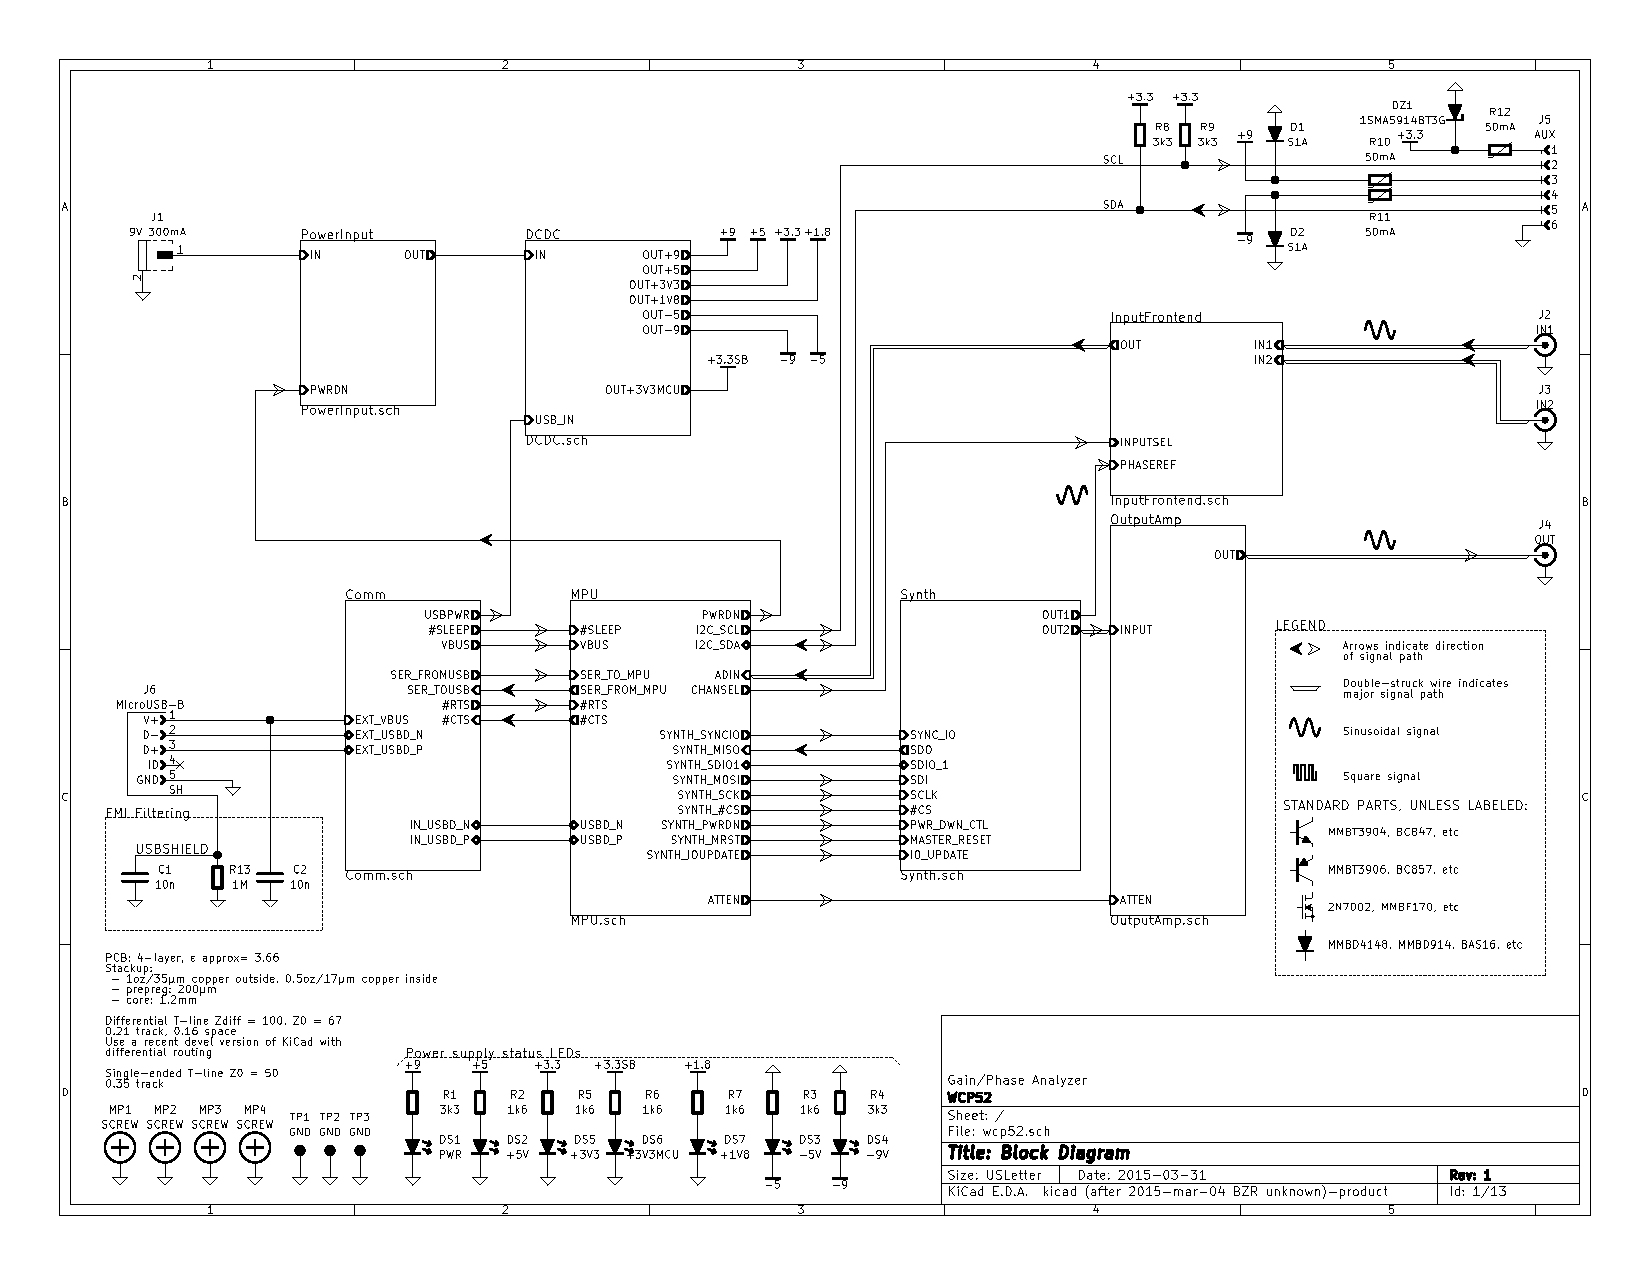
\includepdf[landscape=true,pages=-,link]{schematic.pdf}
\newpage
\begin{thebibliography}{9}

\bibitem{aod417}
Alpha \& Omega Semiconductor, ``AOD417 P-Channel Enhancement Mode Field Effect Transistor,''
AOD417 datasheet, 2008. \url{http://aosmd.com/pdfs/datasheet/AOD417.pdf}

\bibitem{tranckts-sawtooth}
S. W. Amos and M. James, ``Sawtooth generators,'' in
\emph{Principles of Transistor Circuits}, 9th ed. Oxford: Newnes, 2003, ch. 14, pp. 281--292.

\bibitem{az1117c}
Diodes Incorporated, ``Low Dropout Linear Regulator,'' AZ1117C datasheet,
October 2014 [Revision 3--2].
\url{http://www.diodes.com/datasheets/AZ1117C.pdf}

\bibitem{aoe-vreg}
P. Horowitz and W. Hill, ``Voltage regulators and power circuits,'' in
\emph{The Art of Electronics}, 2nd ed. Cambridge: Cambridge, 1989, ch. 6, pp. 307--389.

\bibitem{mcp1700}
Microchip Technology, ``Low Quiescent Current LDO,'' MCP1700 datasheet,
October 2013 [Revision C].
\url{http://ww1.microchip.com/downloads/en/DeviceDoc/20001826C.pdf}

\bibitem{mc79m00}
ON Semiconductor, ``500 mA Negative Voltage Regulators,'' MC79M00 series datasheet,
July 2013 [Revision 15].
\url{http://www.onsemi.com/pub_link/Collateral/MC79M00-D.PDF}.

\bibitem{l78m05}
STMicroelectronics, ``Precision 500 mA regulators,'' L78M datasheet, June 2014 [Revision 20].
\url{http://www.st.com/web/en/resource/technical/document/datasheet/CD00000447.pdf}

\bibitem{tl431}
Texas Instruments, ``TL43xx Precision Programmable Reference,''
TL431 datasheet, Aug. 2004 [Revised Jan. 2015]. \url{http://www.ti.com/lit/ds/symlink/tl431.pdf}

\bibitem{buckinv}
J. Tucker, ``Using a buck converter in an inverting buck-boost topology,''
\emph{Analog Applications Journal}, Texas Instruments, fourth quarter 2007, pp. 16--19.
\url{http://www.ti.com/lit/an/slyt286/slyt286.pdf}
\end{thebibliography}


\begin{appendices}
    \newpage \chapter{Project Requirements}
\label{chap:prs}

\section*{3.1: Required States and Modes}

This system requires the following modes:

\subsection*{3.1.1: Idle}
\label{prs:3.1.1}
The signal source and detection subsystems are inactive, and the system is waiting for commands.

\subsection*{3.1.2: Analysis}
\label{prs:3.1.2}
The system is performing a gain/phase analysis.

\section*{3.2: System Capability Requirements}

\subsection*{3.2.1: Bode plot}
\label{prs:3.2.1}
The analyzer shall be able to display a plot on the operator's PC in the form of a Bode plot.

\subsection*{3.2.2: Test signal frequency}
\label{prs:3.2.2}
The analyzer shall be capable of sourcing test signals between $1$~kHz and $150$~MHz.
(Not applicable: state \hyperref[prs:3.1.1]{WCP52-3.1.1 --- idle})

\subsection*{3.2.3: Test signal amplitude}
\label{prs:3.2.3}
The analyzer shall be capable of output amplitudes up to $1.25$~V~RMS at frequencies up to
$100$~MHz. (Not applicable: state \hyperref[prs:3.1.1]{WCP52-3.1.1 --- idle})

\subsection*{3.2.4: Sensitivity}
\label{prs:3.2.4}
The analyzer shall be able to detect signals down to at least $40$~dB below the output
amplitude. (Not applicable: state \hyperref[prs:3.1.1]{WCP52-3.1.1 --- idle})

\subsection*{3.2.5: Extended sensitivity}
\label{prs:3.2.5}
The analyzer should be able to detect signals down to at least $60$~dB below the output
amplitude. (Not applicable: state \hyperref[prs:3.1.1]{WCP52-3.1.1 --- idle})

\subsection*{3.2.6: Accuracy}
\label{prs:3.2.6}
Amplitude accuracy shall be within $3$~dB, and phase accuracy within $5\dg$.

\subsection*{3.2.7: Extended accuracy}
\label{prs:3.2.7}
Amplitude accuracy should be within $1$~dB, and phase accuracy within $1\dg$, for
frequencies less than $20$~MHz.

\subsection*{3.2.8: Interface safety}
\label{prs:3.2.8}
The hardware shall not be able to be damaged by its remote interface, unless an ``unlock'' command
has been issued.

\section*{3.3: System External Interface Requirements}

\subsection*{3.3.1: Interface}
\label{prs:3.3.1}
The analyzer shall interface with a PC.

\subsection*{3.3.2: Communications type}
\label{prs:3.3.2}
The analyzer should use a text-driven protocol.

\subsection*{3.3.3: Communications medium}
\label{prs:3.3.3}
The analyzer should use a common, standard communication protocol, for example, USB-CDC.

\subsection*{3.3.4: Panel connectors}
\label{prs:3.3.4}
The analyzer shall use either SMA or BNC connectors to interface to the device under test (DUT).

\subsection*{3.3.5: Auxiliary connector}
\label{prs:3.3.5}
The analyzer shall provide power via a front-panel connection for use with external DUT
adapters. The voltage should be at least $\pm 7$~V, and up to $40$~mA should be available.

\section*{3.4: System Internal Interface Requirements}
All internal interfaces are left to the system designers.

\section*{3.5: System Internal Data Requirements}
All decisions about internal data are left to the system designers.

\section*{3.6: Other System Requirements}

\subsection*{3.6.1: Operator's Manual}
\label{prs:3.6.1}
The system should include a simple operator's manual, which should include a brief
Theory of Operation explaining its design, instructions for using each function,
and example test setups for characterization of filters and control loops.

\subsection*{3.6.2: Protocol Guide}
\label{prs:3.6.2}
The system shall include a protocol guide, showing how to communicate with it.

\subsection*{3.6.3: SMT}
\label{prs:3.6.3}
The PCB shall be produced using surface-mount technology as much as is reasonable,
without no-lead packages unless absolutely required.

\subsection*{3.6.4: Direct control}
\label{prs:3.6.4}
The interface should expose direct control of the hardware functions, allowing additional
features to be implemented.

\subsection*{3.6.5: Electrical safety}
\label{prs:3.6.5}
The system shall have no voltages greater than $30$~V peak-to-peak accessible
externally.

\section*{3.7: Precedence and Criticality of Requirements}

All requirements have equal weight.

    \newpage \chapter{Test Procedures}
\label{chap:test}

\section*{3.1.1: Required mode: Idle}
The idle state of the signal source is to be verified by viewing the signal from the
``output'' connector on an oscilloscope. Any signal present must be less than 5~V peak to peak.

The idle state of the detection subsystem is verified by viewing the status annunciators on
the printed circuit board. The annunciator designated ``sample'' must not light.


\section*{3.1.2: Required mode: Analysis}
This requirement is satisfied peripherally by the completion of \hyperref[tp:3.2.6]{requirement 3.2.6}.

\section*{3.2.1: Bode plot}
\label{tp:3.2.1}
\label{tp:3.2.6}
Cause the software to display any data, and verify that it is in the form of a Bode plot.
This means that there should be two plots, both with a horizontal axis of `frequency',
one with a vertical axis of `gain' in decibels, and one with a vertical axis of `phase'
in degrees.

This data can be generated by the instrument (satisfying this requirement peripherally
by the completion of \hyperref[tp:3.2.6]{requirement 3.2.6}), or by any other means.

\section*{3.2.2: Test signal frequency}
\label{tp:3.2.2}
To test this requirement, connect a patch cable between the ``Output'' connector and an oscilloscope
with at least $150$~MHz bandwidth. Either using the PC software or manual control via a serial
terminal, command the instrument to generate signals with frequencies of 1~kHz, 10~MHz, 75~MHz,
and 150~MHz. Using the oscilloscope's frequency display, verify that each signal's frequency is
within 2.5~\% of its nominal value.

\section*{3.2.3: Test signal amplitude}
To test this requirement, connect a patch cable between the ``Output'' connector and an
oscilloscope with at least $300$~MHz bandwidth. Either using the PC software or manual control
via a serial terminal, command the instrument to generate signals with frequencies of
1~kHz, 20~MHz, and 100~MHz, all with maximum amplitude. Using the oscilloscope's amplitude
display, verify that all signals have an amplitude of at least 1.25~V~RMS.

\section*{3.2.4: Sensitivity}
\label{tp:3.2.4}
\begin{enumerate}
\item{Connect a patch cable between ``Output'' and ``Input 1''.}
\item{Command instrument to generate a signal of 100~kHz and maximum amplitude.}
\item{Query reported amplitude.}
\item{Remove patch cable, query reported amplitude. This noise floor must be at least 45~dB
    lower than the amplitude in step 3.}
\item{Reinstall patch cable with a 40~dB attenuator in series. The \Neg 40~dB signal must
    be visible.}
\end{enumerate}

\section*{3.2.5: Extended sensitivity}
To test this optional requirement, perform the same test as in \hyperref[tp:3.2.4]{requirement 3.2.4},
but verify that the final reported amplitude is at least $65\;\mr dB$ lower than the first reported amplitude.

\section*{3.2.6: Accuracy}
\label{tp:3.2.6}

\subsection*{Amplitude}
Connect a pair of patch cables in series using a cable coupler,
and connect this pair between the ``Output'' connector and the ``Input 1'' connector. Configure
the PC software for a full sweep from 1~kHz to 150~MHz not including phase analysis.
Perform normalization. Then, remove the cable coupler and insert a 50~\Ohm{} attenuator with
specified attenuation between 5~dB and 15~dB and bandwidth of at least 200~MHz.
Perform analysis. Verify that the reported gain is within 3~dB of the specified gain of the
attenuator at all frequencies.

\subsection*{Phase}
Connect a patch cable with length under 150~mm between ``Output'' and ``Input 1''.
Configure for a sweep from 10~kHz to 25~MHz, normalize. Using an SMA coupler, add a
patch cable made from 1~m of RG-316 coaxial cable in series. This cable is expected
to exhibit the following phase shift due to propagation delay:

\begin{tabular}{|l|l|}
\hline
Frequency & Phase shift \\ \hline \hline
10~kHz & 0.02\dg \\ \hline
1~MHz & 1.74\dg \\ \hline
10~MHz & 17.4\dg \\ \hline
25~MHz & 43.5\dg \\ \hline
\end{tabular}

Ensure that the propagation delay reported is within 5\dg{} of this at these frequencies.

\section*{3.2.7: Extended accuracy}
To test this optional requirement, perform the test for \hyperref[tp:3.2.6]{requirement 3.2.6},
with the following modifications: the upper sweep limit should be $20$~MHz, reported gain must be
within $1$~dB of the specified attenuator gain, and phase shift must be within $1\dg$ of zero
(above $-1\dg$ and below $+1\dg$) at all frequencies.

\section*{3.2.8: Interface safety}
\label{tp:3.2.8}
To test this requirement, use the interface control commands to attempt to set a GPIO pin
which serves as a signal input to be an output instead. The system must respond with an error.

\section*{3.3.1: Interface}
This requirement is satisfied peripherally by the completion of requirements \hyperref[tp:3.2.1]{3.2.1}
through \hyperref[tp:3.2.8]{3.2.8}, which all required PC interfacing to complete.

\section*{3.3.2: Communications type}
\label{tp:3.3.2}
To test this requirement, connect the instrument to a PC. Connect a serial terminal application
to it, and perform at least one command that produces a response. Demonstrate that the
command and response comprise displayable text symbols.

\section*{3.3.3: Communications medium}
This requirement is demonstrated peripherally as part of demonstrating
\hyperref[tp:3.3.2]{requirement 3.3.2}: the ability for a standard serial console
to talk to the instrument demonstrates that the instrument was using a standard
protocol.

\section*{3.3.4: Panel connectors}
To test this requirement, observe the front panel of the device, and see that the RF connectors are either
SMA or BNC.

\section*{3.3.5: Auxiliary connector}
Using a multimeter, measure all pins on the ``Auxiliary'' connector, verifying that there are
power supply pins with a voltage present of at least \Pos 7~V and \Neg 7~V.
$-7\;\mr V$. Then, switch the multimeter to ammeter mode, and connect in series a selected resistor. Probe
these pins again, and verify that at least $40\;\mr mA$ is supplied.

The resistor is to be selected such that it will draw at least $40\;\mr mA$ at the voltage that was
measured on the connectors. This resistance may depend on the actual voltage that was present,
which is allowed to be \emph{above} the required $\pm 7\;\mr V$.

\section*{3.6.1: Operator's Manual}
Demonstrate the existence of a manual in digital format, containing at least the following
sections: Theory of Operation, Operational Instructions. Demonstrate that there exist example
test setups for characterization of filters and of control loops.

\section*{3.6.2: Protocol Guide}
Demonstrate the existence of documentation explaining the protocol with which a PC communicates with the
instrument. This documentation may be part of the Operator's Manual, or it may be separate.

\section*{3.6.3: SMT}
Demonstrate that the parts on the PCB are surface-mount devices, with the following allowed
exceptions:
\begin{itemize}
\item{Connectors: through-hole connections have higher mechanical stability}
\item{Inductors and capacitors larger than $5\;\mr{mm}$ in diameter: through-hole parts have higher mechanical stability}
\end{itemize}

Demonstrate that the only leadless devices on the PCB are essential for its function. This may be
a result of directly satisfying an above requirement. An anticipated example is device \refdes{U3},
an Analog Devices AD9958BCPZ digital frequency synthesizer, which directly satisfies
\hyperref[tp:3.2.2]{requirement 3.2.2} (test signal frequency between $1\;\mr{kHz}$ and $150\;\mr MHz$).

\section*{3.6.4: Direct control}
Viewing the protocol guide, demonstrate the existence of:

\begin{itemize}
\item{A command to set the output value of an arbitrary GPIO pin.}
\item{A command to query the input value of an arbitrary GPIO pin.}
\item{A command to transmit arbitrary data via the on-board SPI interface.}
\item{A command to query the direct output value of the analog-to-digital converter.}
\end{itemize}

\section*{3.6.5: Electrical safety}
To test this requirement, connect the ``common'' input of a multimeter to the instrument ground, and
verify that no signals on the ``Auxiliary'' connector are more positive than $15$~V or more negative than $-15$~V.
Then, connect a patch cable between the ``Output'' connector and an oscilloscope. Do not terminate the end. Command
the instrument to generate a frequency of $100$~kHz and maximum amplitude. Using the oscilloscope's amplitude display,
verify that the positive and negative peaks are no more positive than $15$~V and no more negative than
$-15$~V.

    \newpage \chapter{Computer Code}
\begin{verbatim}
10 PRINT "HELLO WORLD"
20 GOTO 10
\end{verbatim}
    \newpage \chapter{CAD Drawings}
\end{appendices}

\end{document}
